\documentclass[notes]{beamer}

\usefonttheme[onlymath]{serif}
%\usepackage{blindtext}

\usepackage{amsmath}
\usepackage{hyperref}
\usepackage[export]{adjustbox}
\usepackage{setspace}
\usepackage{tikz}
\usepackage{tabto}

\AtBeginEnvironment{align*}{\small}

\usetheme{Juliaworkshop}
\usefonttheme[onlymath]{serif}

\pdfstringdefDisableCommands{%
  \def\\{}%
}


\title{\Huge A fresh approach to \\ scientific computing}
%\subtitle{Interview}
\date{Maximilian Ernst, Aaron Peikert, Moritz Ketzer}
%\author{Max Planck Institute for Human Development}
\author{
\includegraphics[width=.49\textwidth]{figures/mpib_logo/MPIB_Logo_EN_horizontal_RGB_White.png}}

\setcounter{showSlideNumbers}{1}

\usepackage{svg}
\usepackage{graphicx}
\usepackage{tikz}
\usetikzlibrary{arrows}
\usetikzlibrary{positioning}
\usetikzlibrary{shapes}
\usetikzlibrary{fit}
\usetikzlibrary{backgrounds}

% logo
\logo{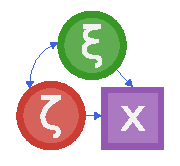
\includegraphics[width=.2\textwidth]{figures/logo_blue.pdf} \hspace{0.22cm}}
\newcommand{\nologo}{\setbeamertemplate{logo}{}} % command to set the logo to nothing
\nologo
\definecolor{mypurple}{RGB}{149, 88, 178}
\newcommand{\monob}[1]{\mbox{\texttt{\textcolor{mypurple}{#1}}}}

\newenvironment{wideitemize}{
    \itemize\addtolength{\itemsep}{15pt}\addtolength{\topsep}{10pt}}{\enditemize}

\newcommand{\A}{\mathbf{A}}
\newcommand{\I}{\mathbf{I}}
\newcommand{\F}{\mathbf{F}}
\newcommand{\OmegaM}{\mathbf{\Omega}}
\newcommand{\SigmaM}{\mathbf{\Sigma}}

\DeclareMathOperator{\prox}{prox}
\DeclareMathOperator*{\argmin}{arg\,min}

\begin{document}
	\setcounter{showProgressBar}{0}
	\setcounter{showSlideNumbers}{0}

	{
	\setbeamertemplate{background}{}
	\setbeamercolor{background canvas}{bg=ExecusharesWhite}
%     \begin{frame}
%         \centering
%         \setstretch{1.5}
%         With every wrinkled face, she sees a story untold, \\
%         Of a life full of laughter, love, and tears, hot and cold, \\
%         She listens with care, to the wisdom they share, \\
%         And learns about the paths that brought them there.\\
%         \hfill \\
%         ChatGPT  \\ (a poem about a PhD candidate in lifespan psychology)
%     \end{frame}
    }

    {
    %\setbeamertemplate{background}{}
	\frame{
	\titlepage}
	}

	%\setcounter{framenumber}{0}
	\setcounter{showProgressBar}{0}
	\setcounter{showSlideNumbers}{0}

	\section{Welcome!}

    \begin{frame}
    \frametitle{Research Software}
    The benefits of R/Python/Matlab \ldots
    \vspace{1cm}
        \begin{wideitemize}
            \item easy to use
            \item packages for everything
            \item large community
        \end{wideitemize}
    \end{frame}

    \begin{frame}
    \frametitle{Research Software}
    The drawbacks of R/Python/Matlab \ldots
    \vspace{1cm}
        \begin{wideitemize}
            \item slow
            \item difficult to extend
        \end{wideitemize}
    \end{frame}

    \begin{frame}
    \frametitle{Speed}
    Traditional divide:
    \vspace{1cm}
        \begin{wideitemize}
            \item compiled languages (C, Fortran, etc \ldots)
            \begin{itemize}
             \item fast, but difficult to work with
            \end{itemize}
            \item scripting languages (R, Python, etc \ldots)
            \begin{itemize}
             \item easy to work with, but slow
            \end{itemize}
        \end{wideitemize}
    \end{frame}

    \begin{frame}
    \frametitle{Speed}
    $\rightarrow$ Two language problem:
        \begin{itemize}
            \item frontend: scripting language
            \item backend: compiled language
        \end{itemize}
    \vspace{1cm}
    For example Numpy (Python) or Dplyr (R)
    \end{frame}
    \begin{frame}
    \frametitle{Speed}
    $\rightarrow$ Julia solves this problem!
    \vspace{1cm}
        \begin{wideitemize}
            \item easy to use syntax
            \item compiled for efficiency
        \end{wideitemize}
    \vspace{1cm}
    ``Walks like Python, runs like C''
    \end{frame}

    \begin{frame}
    \frametitle{Extensibility}
    R/Python packages are typically open source \ldots\\[1cm]
    \only<2->{But the harsh reality is \ldots \\[1cm]}

    \begin{wideitemize}
        \item<3-> \textbf{understand} 1000s of lines of code
        \item<4-> make \textbf{changes}, possibly breaking stuff
    \end{wideitemize}
    \end{frame}

    \begin{frame}
        \frametitle{Extensibility}
        $\rightarrow$ Julia solves this problem too!\\[1cm]
        You are able to add new features...
        \vspace{0.8cm}
        \begin{wideitemize}
            \item<1-> without \textbf{understanding} existing code
            \item<2-> without \textbf{changing} existing code
        \end{wideitemize}
    \end{frame}

	\section{This Workshop}

    \begin{frame}
        \frametitle{This Workshop}
        \begin{wideitemize}
            \item focuse on extensibility (performance comes almost for free)
            \item design principles of the julia language
            \item self-paced
        \end{wideitemize}
    \end{frame}

    \section{Questions?}

\end{document}
